\section{Adhoc-Netzwerke}\label{s:AdhocNetzwerke}

Adhoc-Netze sind in sich geschlossene Netzwerke, organisieren sich selbst und haben keine bestimmte Hierarchie. Sie bauen sich nur für die Dauer einer Datenübertragung auf, besitzen keine festgelegte Kommunikationsstruktur und verwalten sich selbst. 

Adhoc-Netze sind leistungsfähige Netzwerke und zählen als so genanntes \ac{SON}, welche gute Lastverteilung betreiben und ohne zentrales Management auskommen. Die Endgeräte übernehmen in diesem Fall das Routing und speichern die Routingtabellen selbst ab. Geräte, die sich dem Netzwerk anschließen, werden dynamisch in das Netz eingefügt. Bei Netzwerken nach IEEE 802.11 (WLANs) und IEEE 802.15 (WPANs - hier im Speziellen IEEE 802.15.1 - Bluetooth) werden alle Geräte selbstständig erkannt und dem Netz hinzugefügt. Sie sind fortan Bestandteil des Gesamtnetzes. 

Bei Adhoc-Netzen mit vielen Geräten (das kann z.B. ein Sensornetz sein) wird zumeist eine Multihop-Verbindung bevorzugt. Das bedeutet, dass die Daten von einem Netzknoten, z.B. einem Sensor oder Rechner, zu dem nächsten Netzknoten weitergeleitet werden, bis sie ihr Ziel erreicht haben. Fällt ein Knoten aus, wird wenn möglich ein anderer Weg für die Übertragung genutzt, um Ausfälle zu vermeiden.

Ad-hoc-Netzwerke bestehen virtuell für einen begrenzten Zeitrahmen. Ad-hoc bedeutet etwa 'für den Augenblick gemacht'. Sie werden in WLANs, WPANs, in Sensornetzen (WPANs mit geringer Datenrate - siehe IEEE 802.15.4) und in Funknetzen von Rettungsdiensten, Polizei und Militär benutzt \cite{ws:lipinski}.

\subsection{MANETs}\label{ss:MANETs}

MANET bezeichnet die Abkürzung für den Begriff 'Mobile Ad-hoc Network‘. Jochen Schiller beschreibt in seiner Literatur 'Mobile Communications' den Begriff des MANETs wie folgt:
 
\begin{quote}
„Ad-hoc-Netze kommen ohne jegliche Infrastruktur aus, insbesondere ohne eine ausgezeichnete Basisstation, welche den Medienzugriff zentral steuert. Diese Netzvariante erlaubt die spontane, nicht vorab geplante Kommunikation zwischen mobilen Endgeräten, wobei einige oder alle Endgeräte auch Daten von anderen Endgeräten weiterleiten können.“
\end{quote}
	
\begin{figure}[H] 
	\centering
	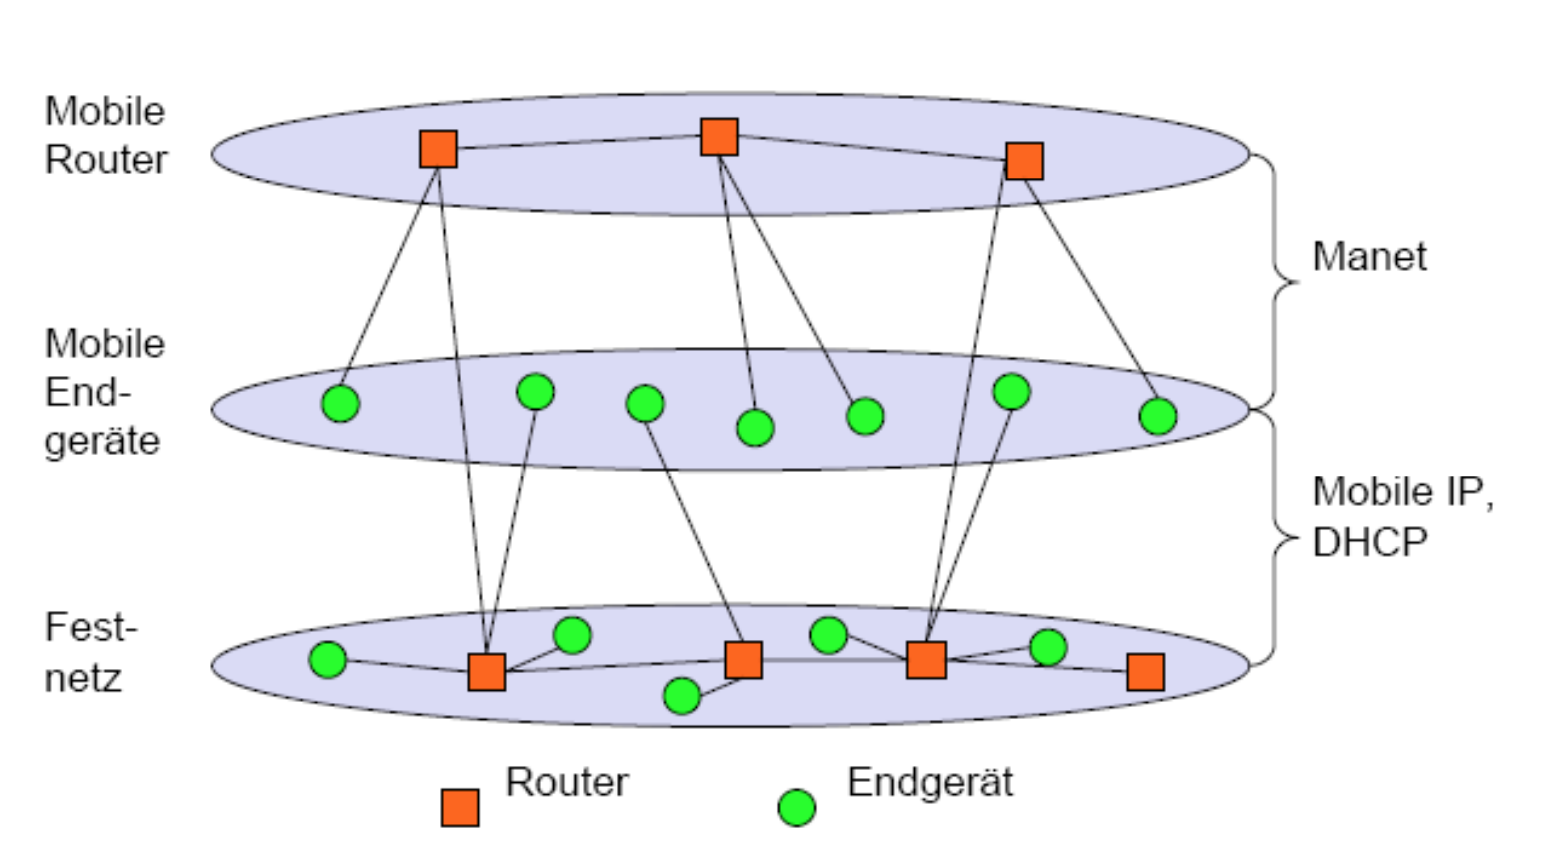
\includegraphics[scale=0.5]{Bilder/manet}
	\caption{Einordnung von MANETs\cite{d:timm}}
	\label{f:manet}
\end{figure}

MANETs zeichnen sich vor allem dadurch aus, dass sie keine feste Infrastruktur besitzen. Es herrscht innerhalb des Netzes eine dynamische Topologie, was bedeutet, dass zu jedem Zeitpunkt bestimmte Knoten wegfallen und neue dazukommen können. Dies führt dazu, dass bislang bekannte und zulässige Routen wegfallen, dafür aber auch neue Routen entstehen können. Unter den Geräten besteht eine spontane Vernetzung. Das bedeutet, dass jedes Gerät sowohl Endpunkt einer Übertragung sein kann, jedoch auch in der Lage sein muss, Daten weiterleiten zu können. Durch dieses Weiterleiten von Daten entsteht eine so genannte 'Multihop-Umgebung‘, da die Daten nicht vom Sender direkt zum Empfänger gelangen, sondern den Empfänger über mehrere Zwischenstationen erreichen. \\

\begin{figure}[H] 
	\centering
	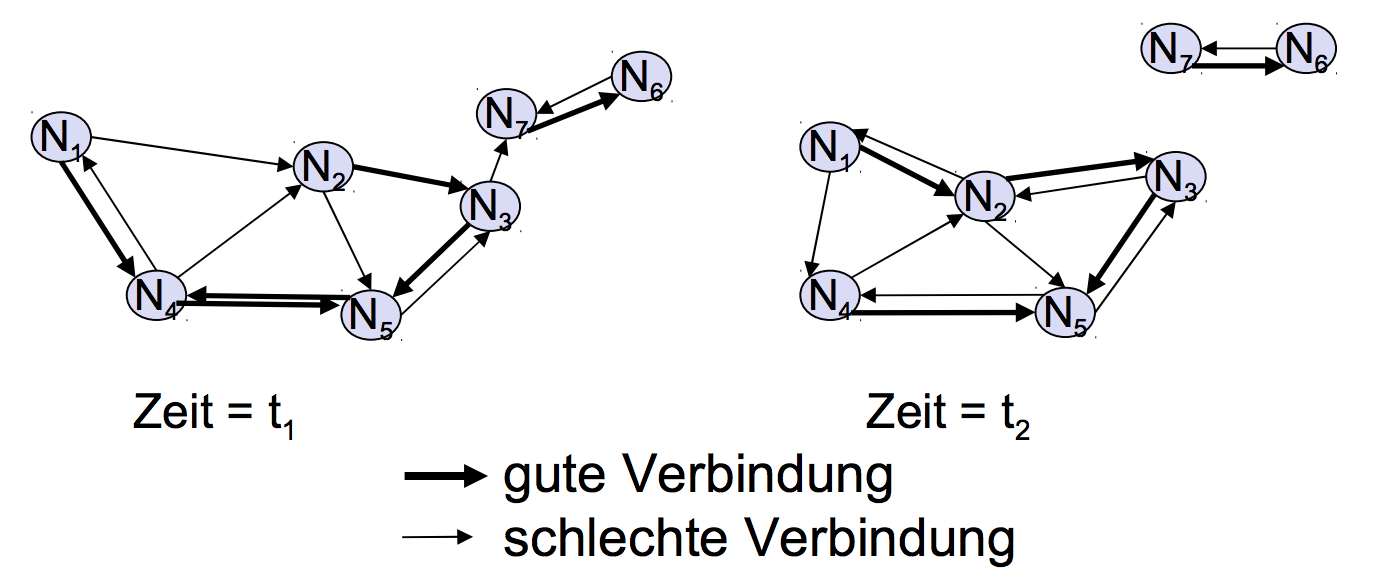
\includegraphics[scale=0.5]{Bilder/manetconnection}
	\caption{Mögliche Verbindungen eines Beispiel MANETs\cite{d:timm}}
	\label{f:manetconnection}
\end{figure}

Mobile Ad-hoc Netzwerke besitzen eine stark begrenzte Bandbreite. Da sie meistens auf stromsparende Übertragungsprotokolle setzen, können dementsprechend auch nur geringe Mengen an Daten übertragen werden. Des Weiteren bestehen zumeist durch die unterschiedlichen Übertragungsleistungen der Geräte asymmetrische Verbindungen, welche sich für die Übertragung von Daten innerhalb des Netzes besser eignen.\\

Ein Problem bei MANETs stellt die beschränkte Möglichkeit der Energieversorgung dar, da die Endgeräte meistens abhängig von Batterien oder Akkus sind. Durch die hohe Menge an Geräten in einem Netz steigt dazu die Summe des potenziellen Energiebedarfes pro Gerät weiter an. Auch die Sicherung des Netzes vor physischen Angriffen ist stark beschränkt. So sind z.B. Denial-of-Service-Attacken (DoS), Überwachungsangriffe oder auch das Verfälschen von Nachrichten oft leicht zu realisieren \cite{d:timm}.

\subsection{Routingprotokolle}\label{ss:Routingprotokolle}

Klassische Routingprotokolle versagen bei dem Versuch, sie innerhalb von mobilen Ad-hoc Netzwerken einzusetzen. Gründe dafür sind folgende: \\

MANETs zeichnen sich durch eine hohe Dynamik aus, das Netz verändert sich spontan, schnell und ständig. Klassische Protokolle besitzen eine zu langsame Konvergenz, um dem Anspruch der sich ständig verändernden Ad-hoc Netze gerecht zu werden und sind somit nicht geeignet.\\

Ad-hoc Netze besitzen wie bereits erwähnt meist eine geringe Bandbreite. Hinzu kommt, dass den angeschlossenen Knoten und Geräten nur eine gewisse Rechenleistung zur Verfügung steht. Sie sind somit mit klassischen Routingprotokollen überfordert, da diese meist viel Rechenleistung und Übertragungsleistung erfordern, welche mit den mobilen Geräten nicht realisierbar sind. Der Overhead der klassischen Protokolle ist also für diese Art von Netzwerken zu groß. \\

Es gibt in mobilen Ad-hoc Netzen gewisse Metriken, die beim Betrieb berück\-sichtigt werden müssen. Die klassischen Protokolle interessieren sich nicht für diese Metriken und lassen sie außen vor. Bei der Auswahl von Routen müssen unter anderem folgende Aspekte betrachtet werden:
\begin{itemize}
	\item Batterielaufzeit der Geräte
	\item Zeit der Verbindung zwischen zwei Geräten
	\item Energiebedarf
	\item Zuverlässigkeit der Verbindung
\end{itemize} 

Zusammengefasst lässt sich sagen, dass Routingprotokolle für MANETs vor allem eine große Skalierbarkeit im Hinsicht auf eine große Anzahl von Geräten, Flexibilität und Effizienz im Hinblick auf Komplexität, Energieverbrauch und Speicherverbrauch erfordern. Diese werden mittlerweile intensiv erforscht, da Ad-hoc Netze im Zusammenhang mit dem 'Internet of Things‘ (IoT) oder auch dem 'Internet Of Everything‘ (IoE) zunehmend an Bedeutung gewinnen \cite{d:timm}. \\

Im Folgenden sollen die Protokolle OLSR, AODV und CGSR kurz aufgezeigt und erklärt werden.

\subsubsection{OLSR}\label{ss:OLSR}

Die Abkürzung OLSR steht für 'Optimized Link State Routing‘ und bezeichnet ein flaches, proaktives Linkstate-Protokoll. Proaktiv bedeutet in diesem Fall, dass in gewissen Zeitabständen automatisch Kontrollnachrichten ausgetauscht werden. Bei einem Linkstate-Protokoll sendet z.B. jeder Router den anderen Knoten im Netz den Zustand der Verbindung zu seinen Nachbarn. \\
Das OLSR-Routingprotokoll ist als \ac{RFC} 3626 spezifiziert und erweitert normale Link-State-Protokolle, in dem die Komplexität jener Protokolle vereinfacht wird. \\
Bei OLSR hat jeder Knoten einen Überblick über alle andere Knoten im Netzwerk und den Routen dort hin, somit kann jeder Knoten seine Routen mit dem 'Shortest Path Algorithm‘ eigenständig errechnen. Allerdings haben nicht alle Knoten die gleichen Bedeutungen und Aufgaben.\\
Um Nachbarknoten zu finden, werden sie mit einer 'Hello-Message‘ gesucht. Die Kontrollpakete werden in entsprechenden Zeitabständen erstellt und enthalten die Knotenadresse, eine Sequenznummer und die Nachbarknoten mit Distanzinformationen. Folglich enthält jeder Knoten die Distanzinformationen von allen anderen Knoten, so kann die Topologie erstellt und die Routen mit o.g. 'Shortest Path Algorithm‘ berechnet werden. \\

Das OLSR unterscheidet sich von anderen Link-State-Algorithmen, da es ein optimiertest Link-State-Routing verwendet. Es werden so genannte 'Multi-Point-Relays‘ ausgewählt und verteilt, was für ein effizienteres Routing sorgt. Die Relays sind im Stande, die Kontrollnachrichten an die angeschlossenen Knoten weiterzuleiten.

\begin{figure}[H] 
	\centering
	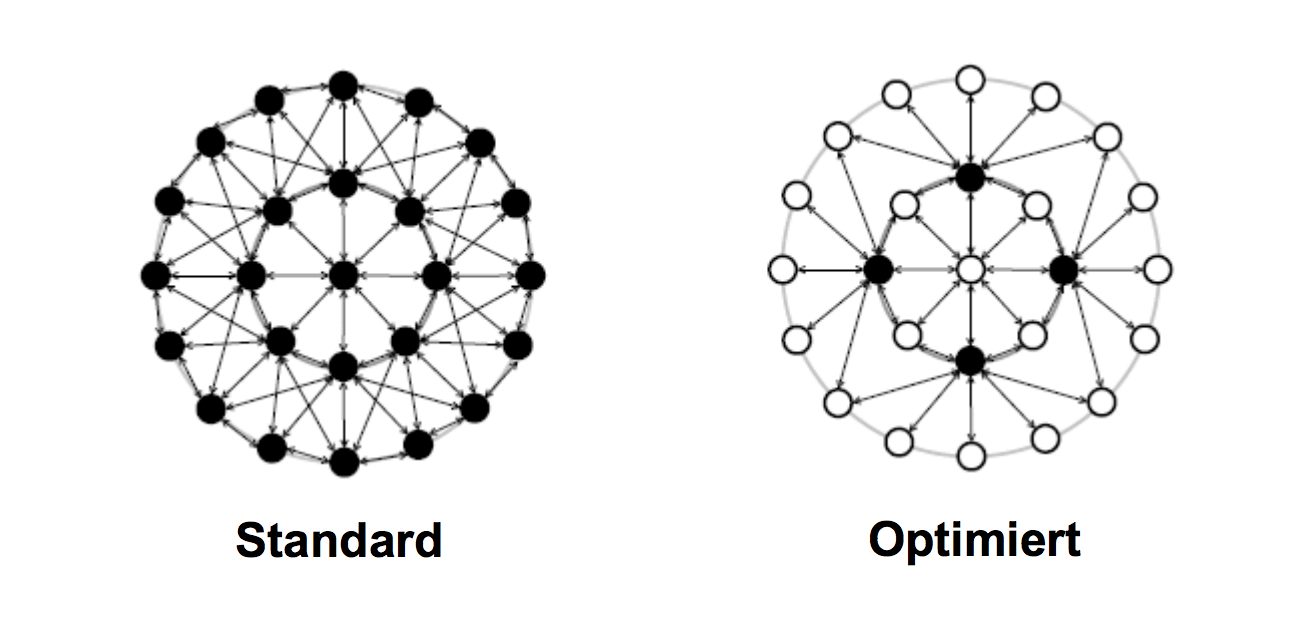
\includegraphics[scale=0.5]{Bilder/olsr}
	\caption{optimiertes LSR durch Multi-Point-Relays im OLSR\cite{d:timm}}
	\label{f:olsr}
\end{figure}

\subsubsection{AODV}\label{ss:AODV}

Das Ad-hoc On-Demand Distance Vector Routingprotokoll ist ein flaches, reaktives Distanzvektorprotokoll. Reaktive Protokolle tauschen im Gegensatz zu proaktiven Protokollen nur Kontrollnachrichten aus, wenn neue Routen benutzt werden sollen. Sie benötigen weniger Bandbreite und sind dynamischer, allerdings besteht nur eine Teilkenntnis des Netzwerks, somit müssen die Routen anders berechnet werden.\newpage
AODV ist in RFC 3561 spezifiziert und für IPv4-Netze vorgesehen. Es erlaubt eine theoretisch unbegrenzte Anzahl von Geräten im Netzwerk. Bei AODV  kennt jeder Knoten nur den 'Next Hop‘, den nächsten Knoten, und die Länge der Gesamtroute. Das Protokoll definiert insgesamt zwei Routingalgorithmen 'Route Discovery‘ und 'Route Maintenance‘.  \\

Bei der 'Route Discovery‘ wird die Route aufgebaut, wozu zwei Nachrichtentypen benötigt werden. Es wird zunächst eine 'Route-Request-Nachricht‘ (RREQ) per Broadcast zum Ziel gesendet. Das Ziel antwortet widerum mit einer 'Route-Reply-Nachricht‘ (RREP) per Unicast zurück an den Absender. Sollte eine bidirektionale Verbindung zwischen zwei Geräten herrschen, wird per Route Discovery auch eine bidirektionale Route aufgebaut. \\

\begin{figure}[H] 
	\centering
	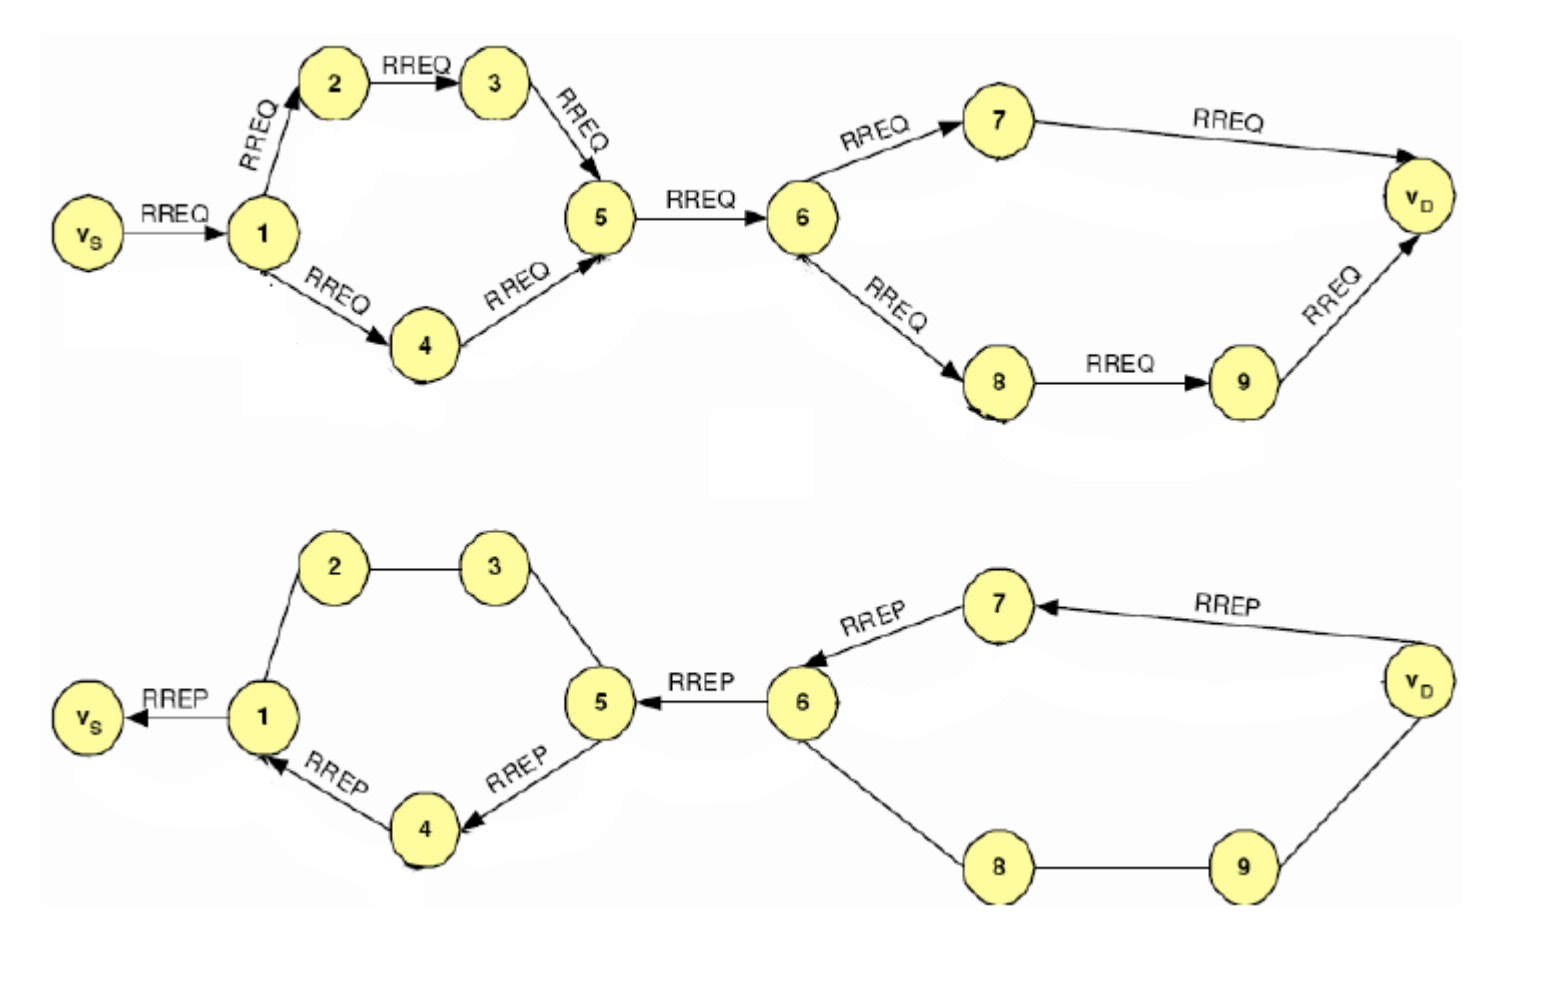
\includegraphics[scale=0.5]{Bilder/aodv}
	\caption{'Route Discovery‘ im AODV-Protokoll\cite{d:timm}}
	\label{f:aodv}
\end{figure}

Bei 'Route Maintenance‘ handelt es sich um die Verwaltung der Routen. Es wird eine 'Route-Error-Nachricht‘ (RRER) versendet, sobald eine defekte Route diagnostiziert wird. Diese Nachricht wird an alle Nachbarn versendet, so dass jeder Knoten über das Wegfallen der Route informiert wird.
\newpage
\subsubsection{CGSR}\label{ss:CGSR}

Beim Clusterhead-Gateway Switch Routing (CGSR) handelt es sich um ein hierarchisches Protokoll, was bedeutet, dass für verschiedene Knoten unterschiedliche Rollen vorgesehen sind. \\
Das Netzwerk wird bei CGSR in Cluster aufgeteilt, die sich allerdings teilweise überdecken müssen. Für jedes dieser Cluster wird ein 'Clusterhead‘ ernannt. Ein Knoten, welcher sich in zwei Clustern gleichzeitig befindet, wird als Gateway bezeichnet.

\begin{figure}[H] 
	\centering
	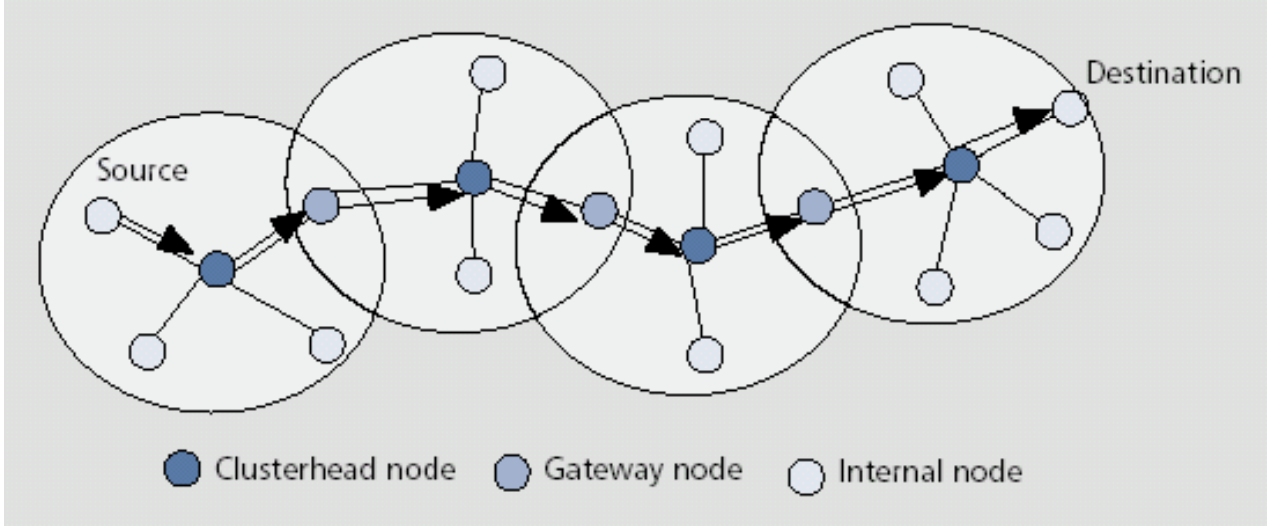
\includegraphics[scale=0.5]{Bilder/cgsr}
	\caption{Clustering im CGSR-Protokoll\cite{d:timm}}
	\label{f:cgsr}
\end{figure}

Das Clusterhead-Gateway Switch Routing basiert auf einem Distanzvektor-Protokoll. Jeder Knoten im Netzwerk speichert sowohl eine Distanzvektor-Routing-tabelle, als auch eine 'Cluster Member‘-Tabelle. Die Distanzvektor-Tabelle enthält neben den normalen Routingeinträgen einen Routingeintrag zum Clusterhead jedes Clusters. In der 'Cluster Member‘-Tabelle wird für jeden Knoten der Clusterhead gespeichert, damit klar ist, welcher Knoten zu welchem Cluster gehört. \\

Der große Vorteil von CGSR besteht in der signifikanten Reduzierung der Größe der Routingtabellen im Vergleich zu anderen Distanzvektorprotokollen, somit ist das CGSR für Ad-hoc Netzwerke dank seiner geringeren Komplexität gut geeignet.

